\documentclass[times]{article}

\usepackage{graphicx}
\usepackage{float}
\usepackage{placeins}
\usepackage[none]{hyphenat}
\usepackage{amsmath}
\usepackage[us]{datetime}
\usepackage[explicit]{titlesec}
\titleformat{\section}{\normalfont}{}{0em}{\textbf{\large Problem  \thesection}\  \normalsize #1}
\begin{document}
	\title{CS 5800 Distributed OS - Spring 2017 \\ Homework 3}
	\author{Josh Herman \\ Dalton Cole \\ Neil Blood}
	\date{\formatdate{7}{3}{2017}}
	\maketitle

	% Question 2
	\section{Show how Dijkstra-Scholten termination detection algorithm worksusing the example graph given in Figure 1 assuming node 0 is the initiator.}
		
		\begin{figure}[H]
			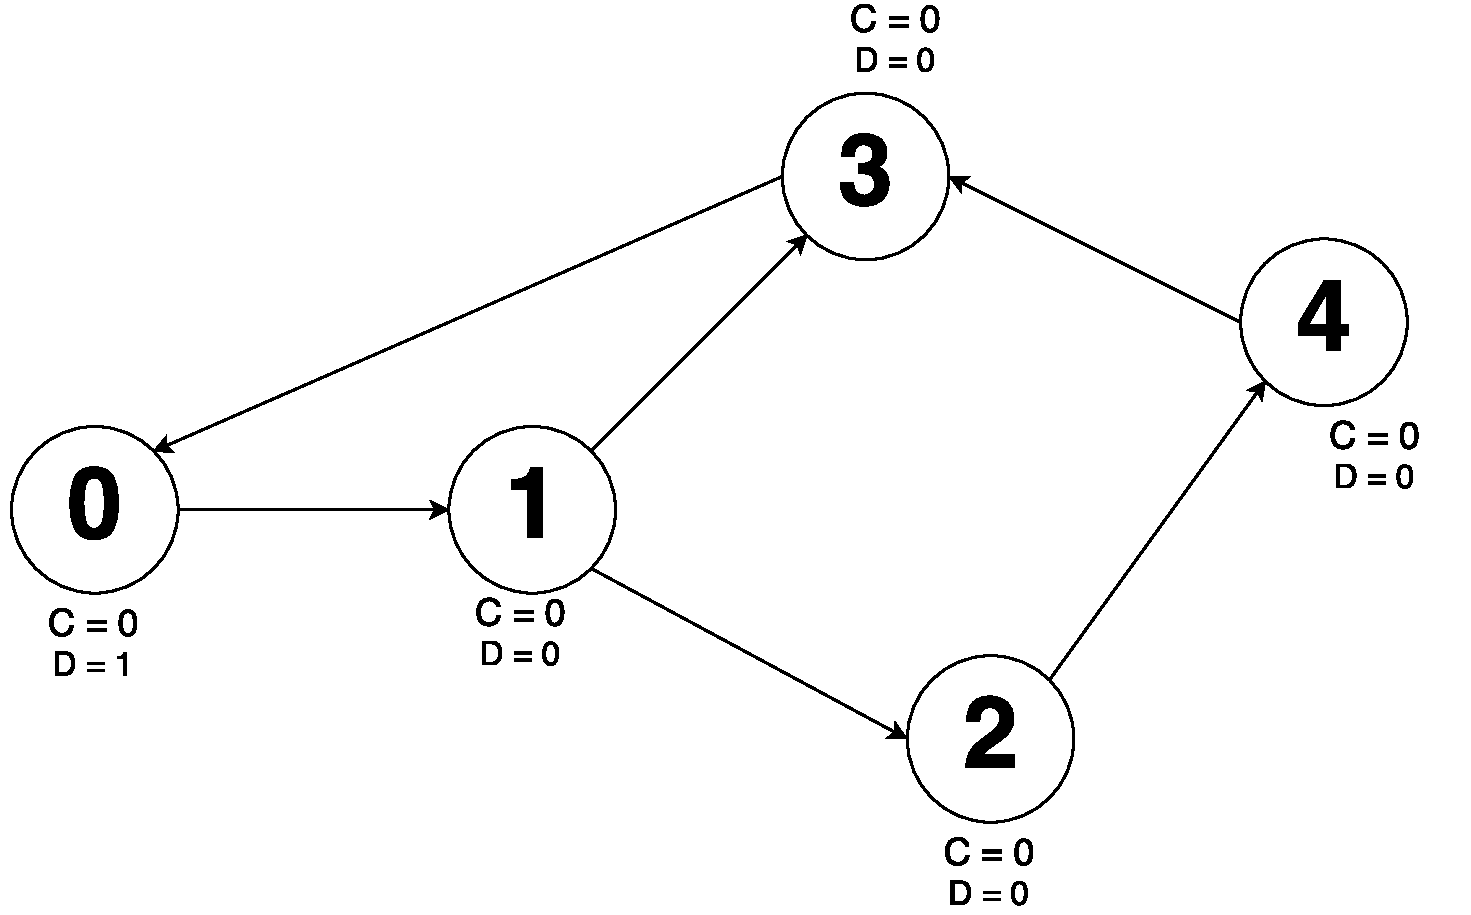
\includegraphics[width=\linewidth]{q2/1.pdf}
		\end{figure}
		\begin{figure}[H]
			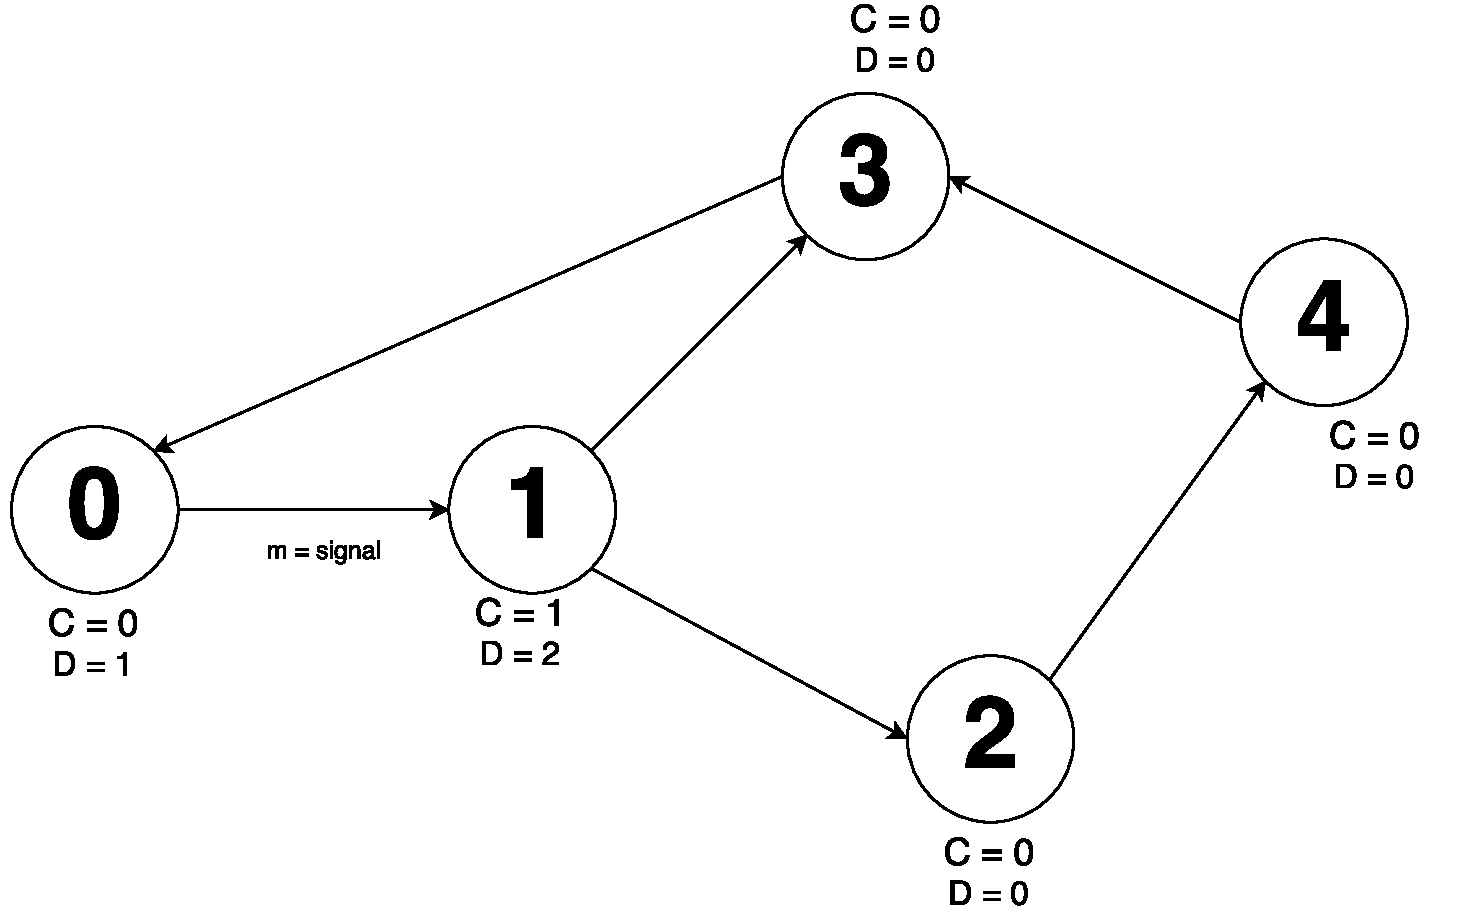
\includegraphics[width=\linewidth]{q2/2.pdf}
		\end{figure}
		\begin{figure}[H]
			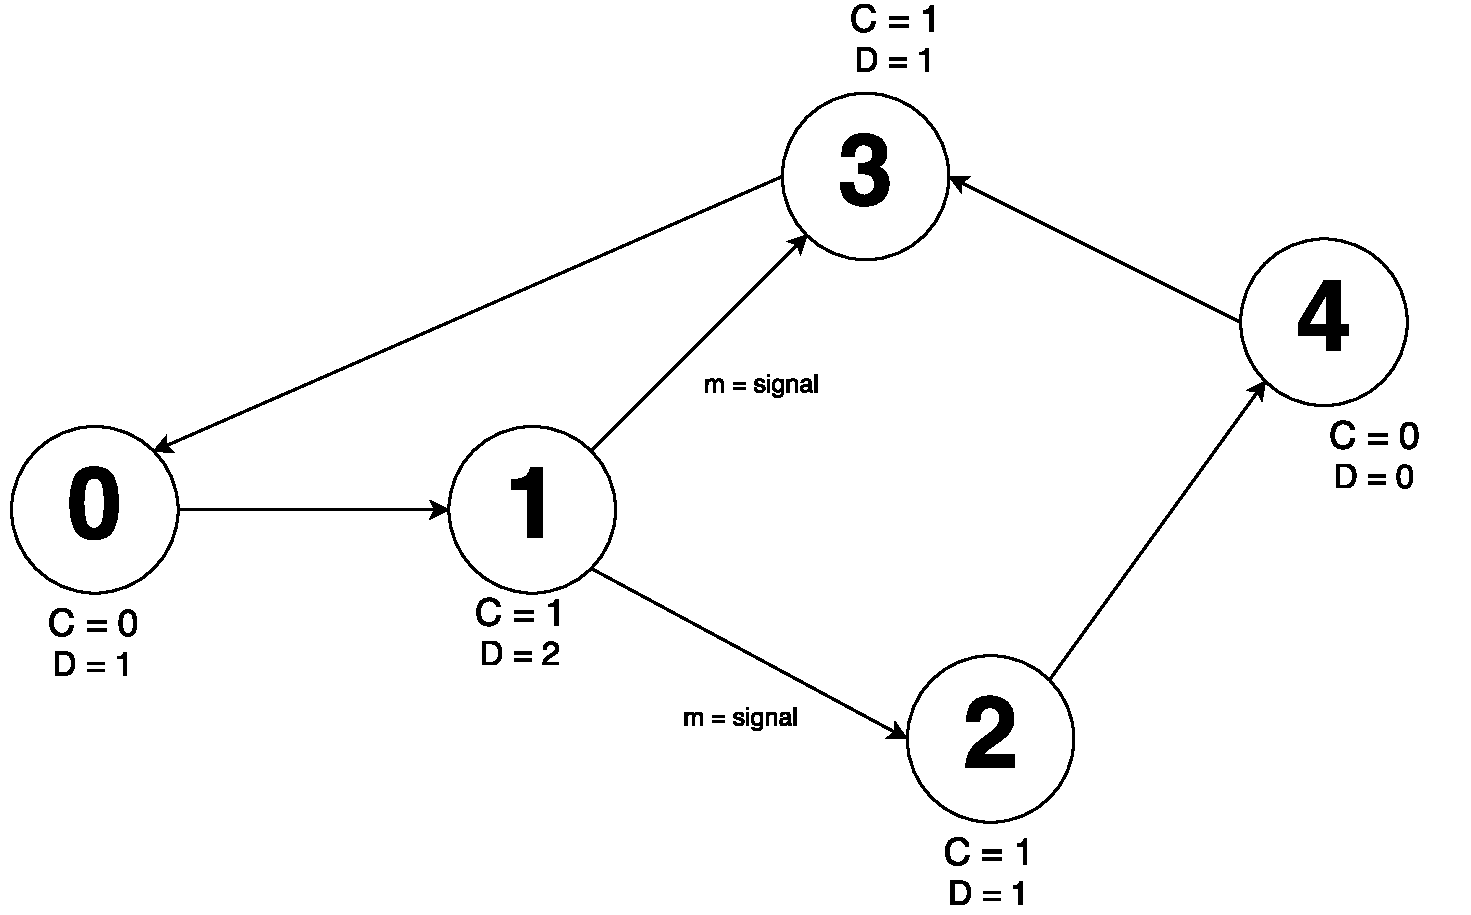
\includegraphics[width=\linewidth]{q2/3.pdf}
		\end{figure}
		\begin{figure}[H]
			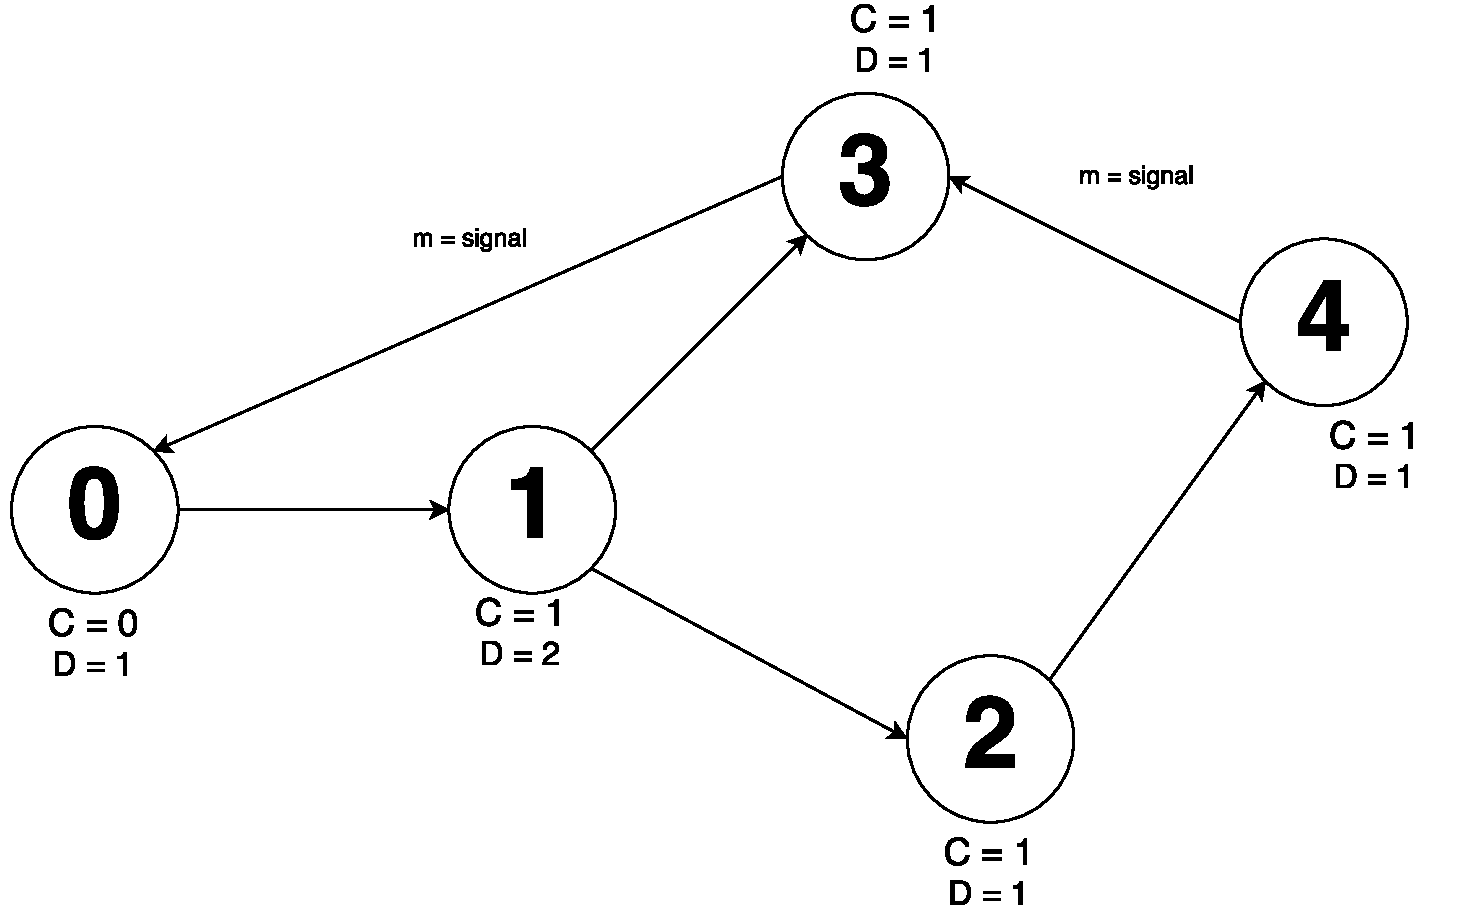
\includegraphics[width=\linewidth]{q2/4.pdf}
		\end{figure}
		\begin{figure}[H]
			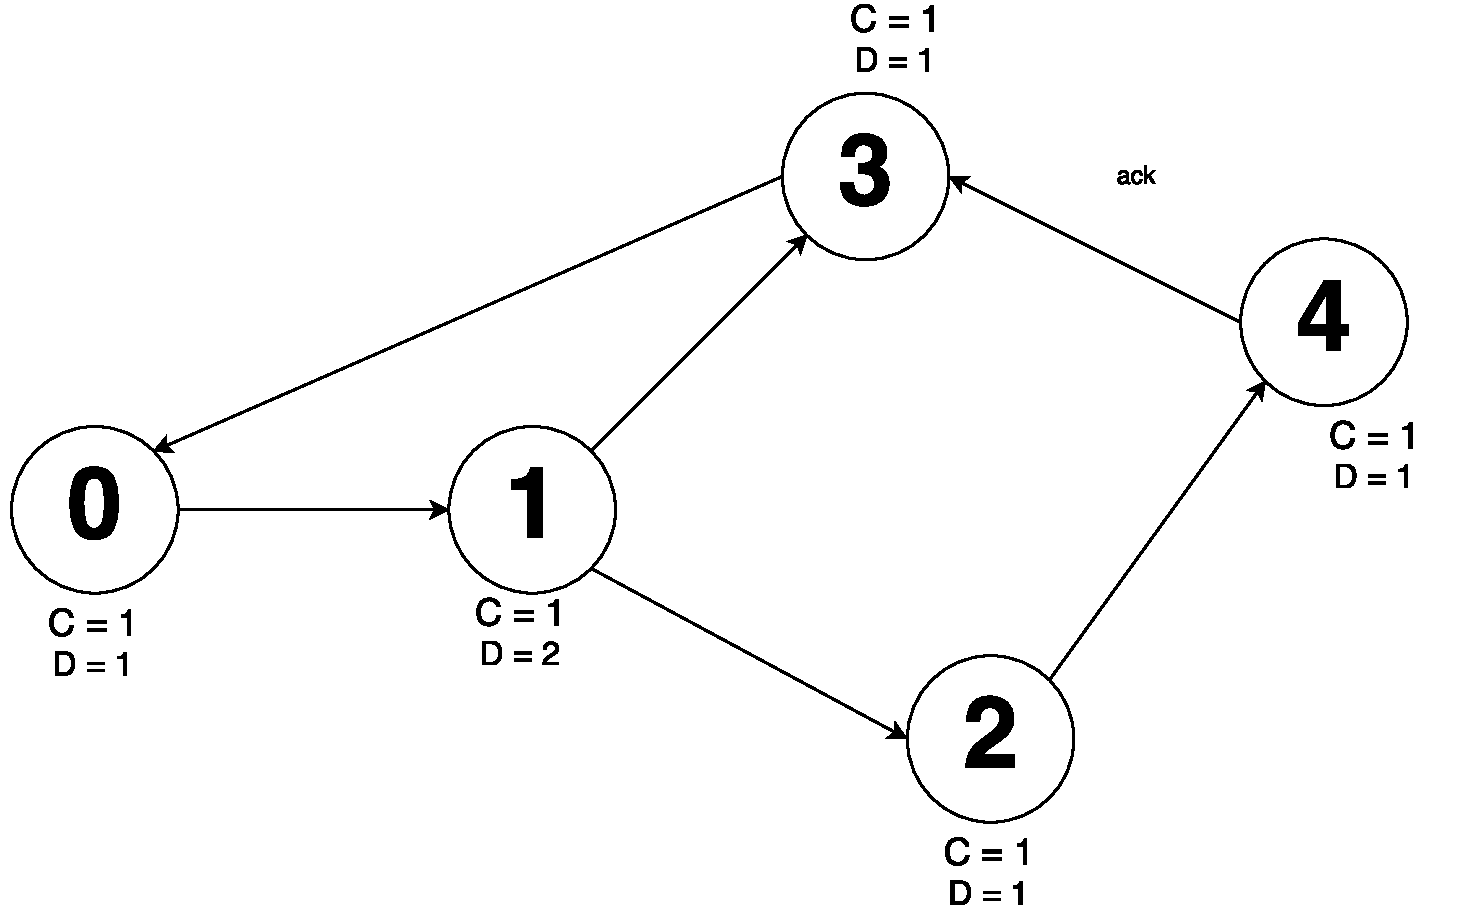
\includegraphics[width=\linewidth]{q2/5.pdf}
		\end{figure}
		\begin{figure}[H]
			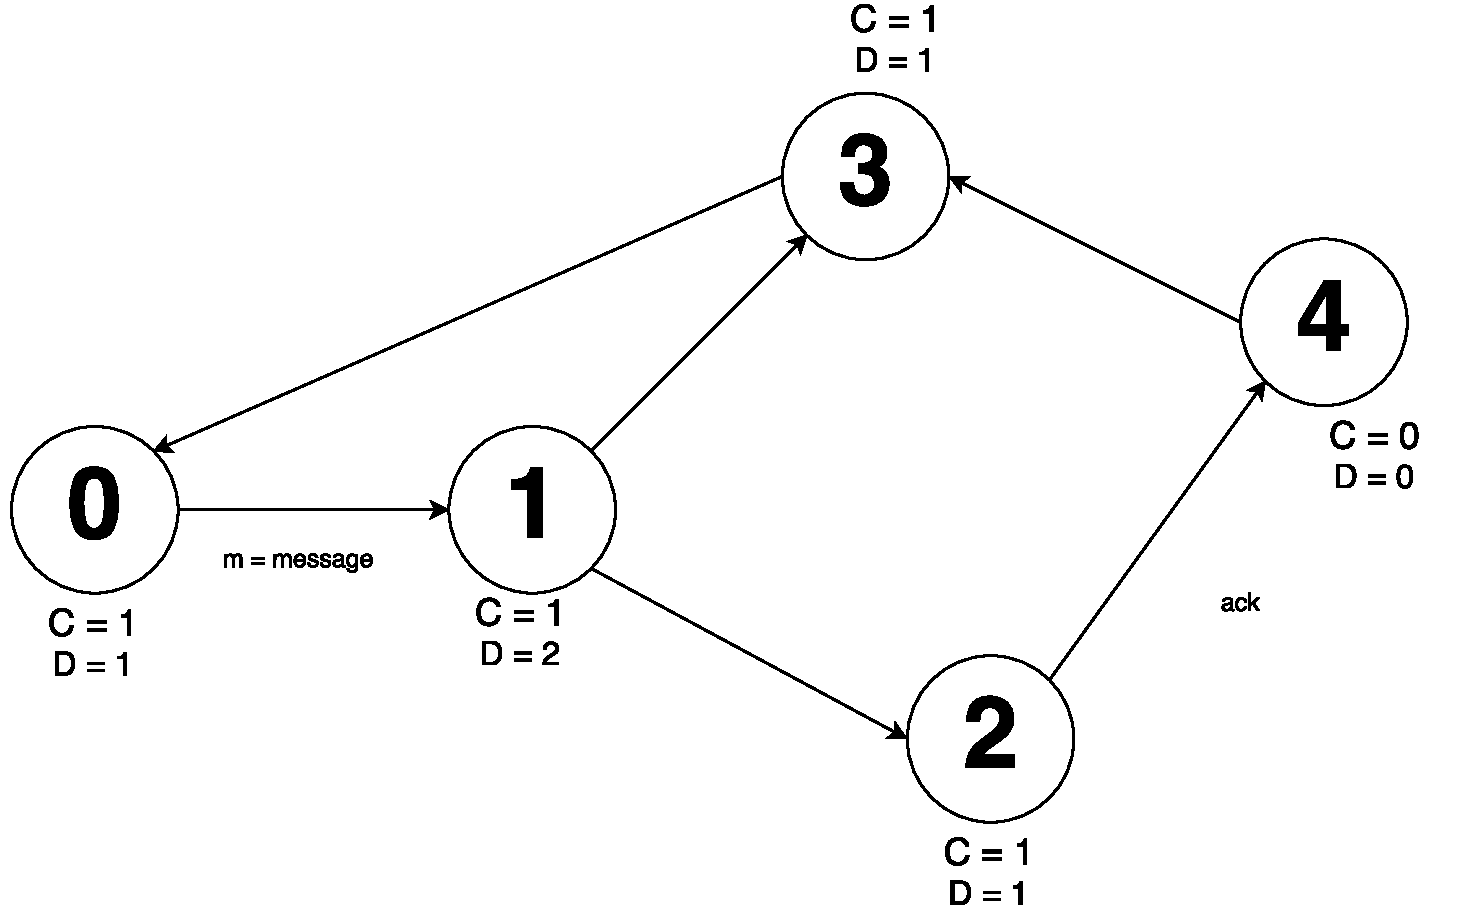
\includegraphics[width=\linewidth]{q2/6.pdf}
		\end{figure}
		\begin{figure}[H]
			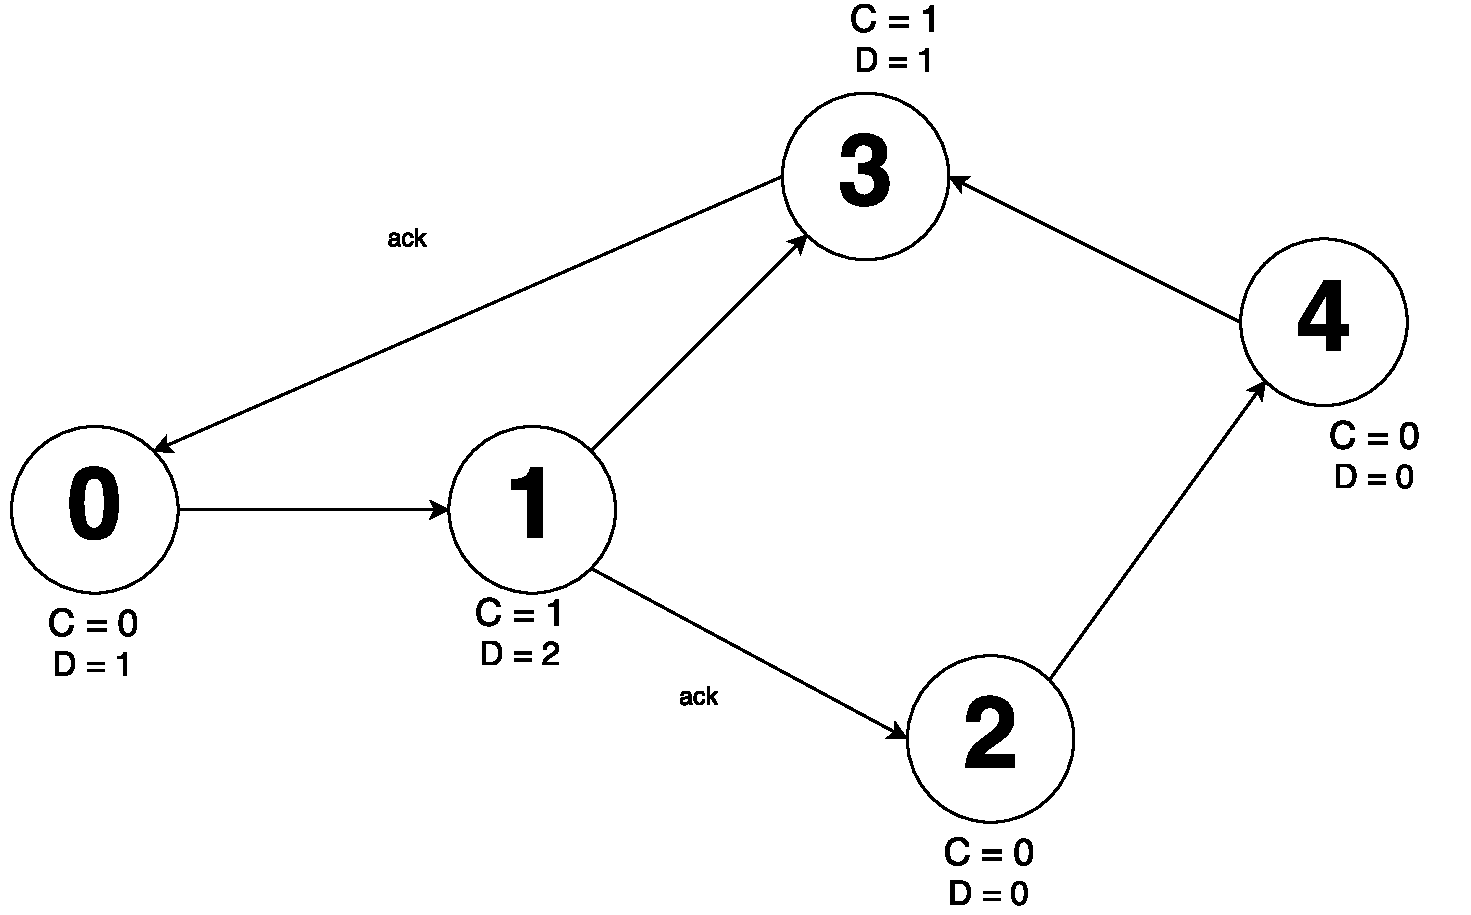
\includegraphics[width=\linewidth]{q2/7.pdf}
		\end{figure}
		\begin{figure}[H]
			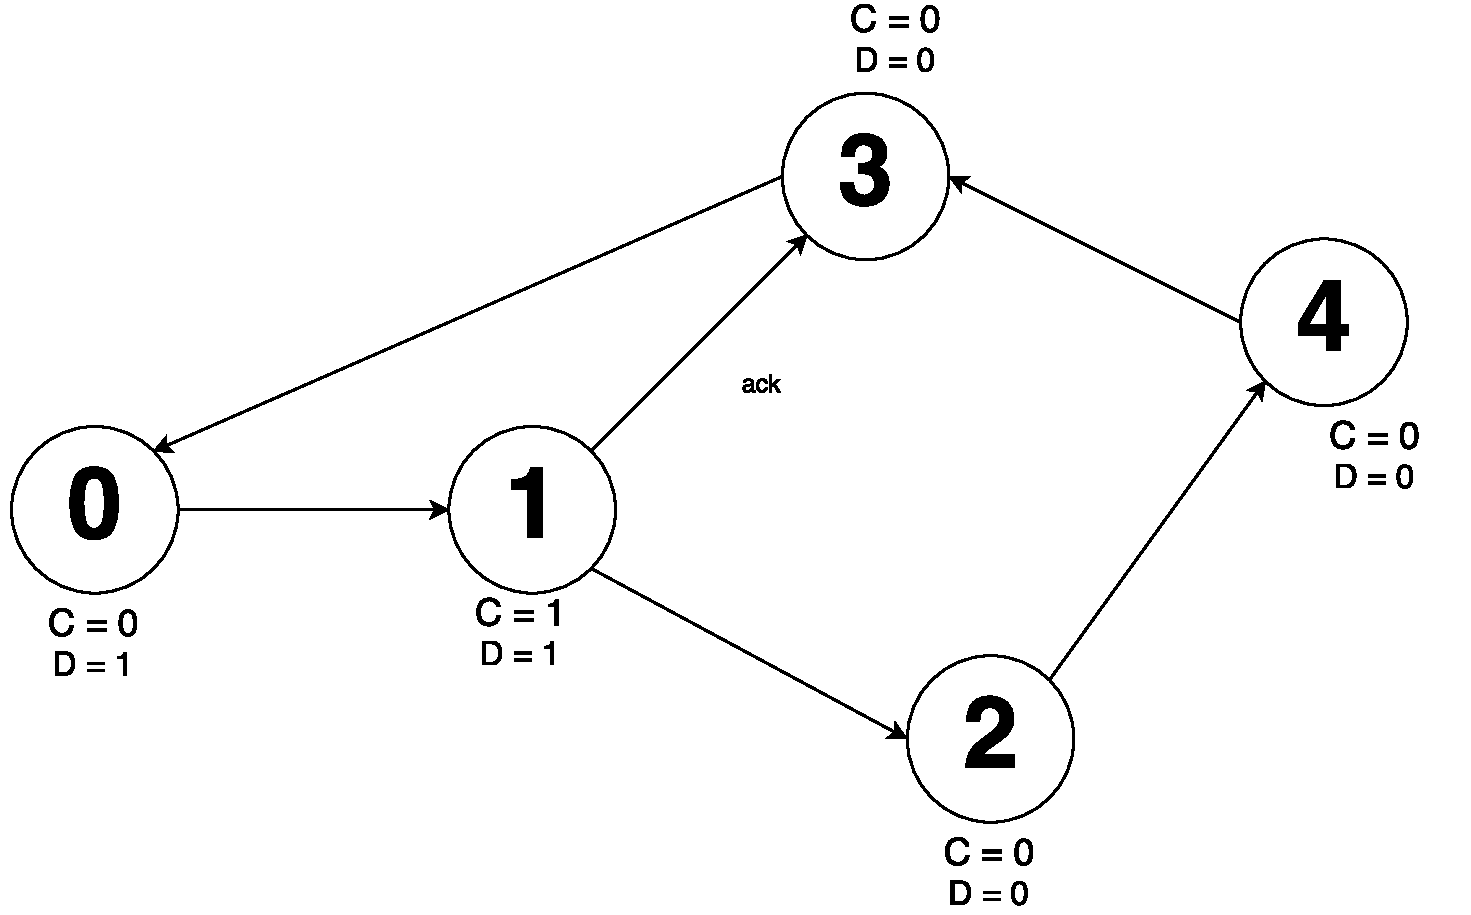
\includegraphics[width=\linewidth]{q2/8.pdf}
		\end{figure}
		\begin{figure}[H]
			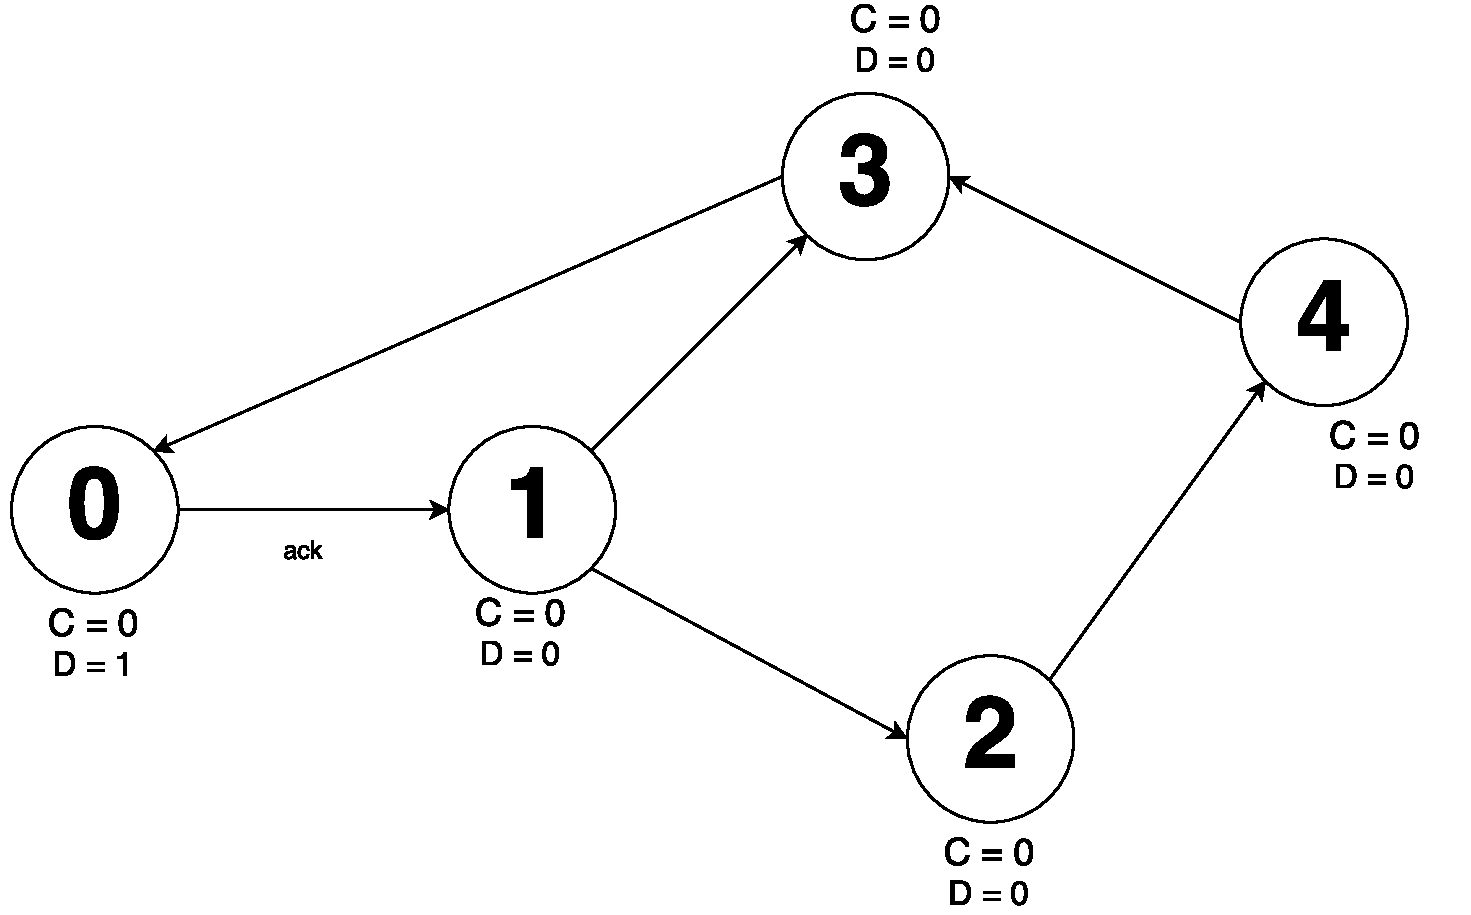
\includegraphics[width=\linewidth]{q2/9.pdf}
		\end{figure}
		\begin{figure}[H]
			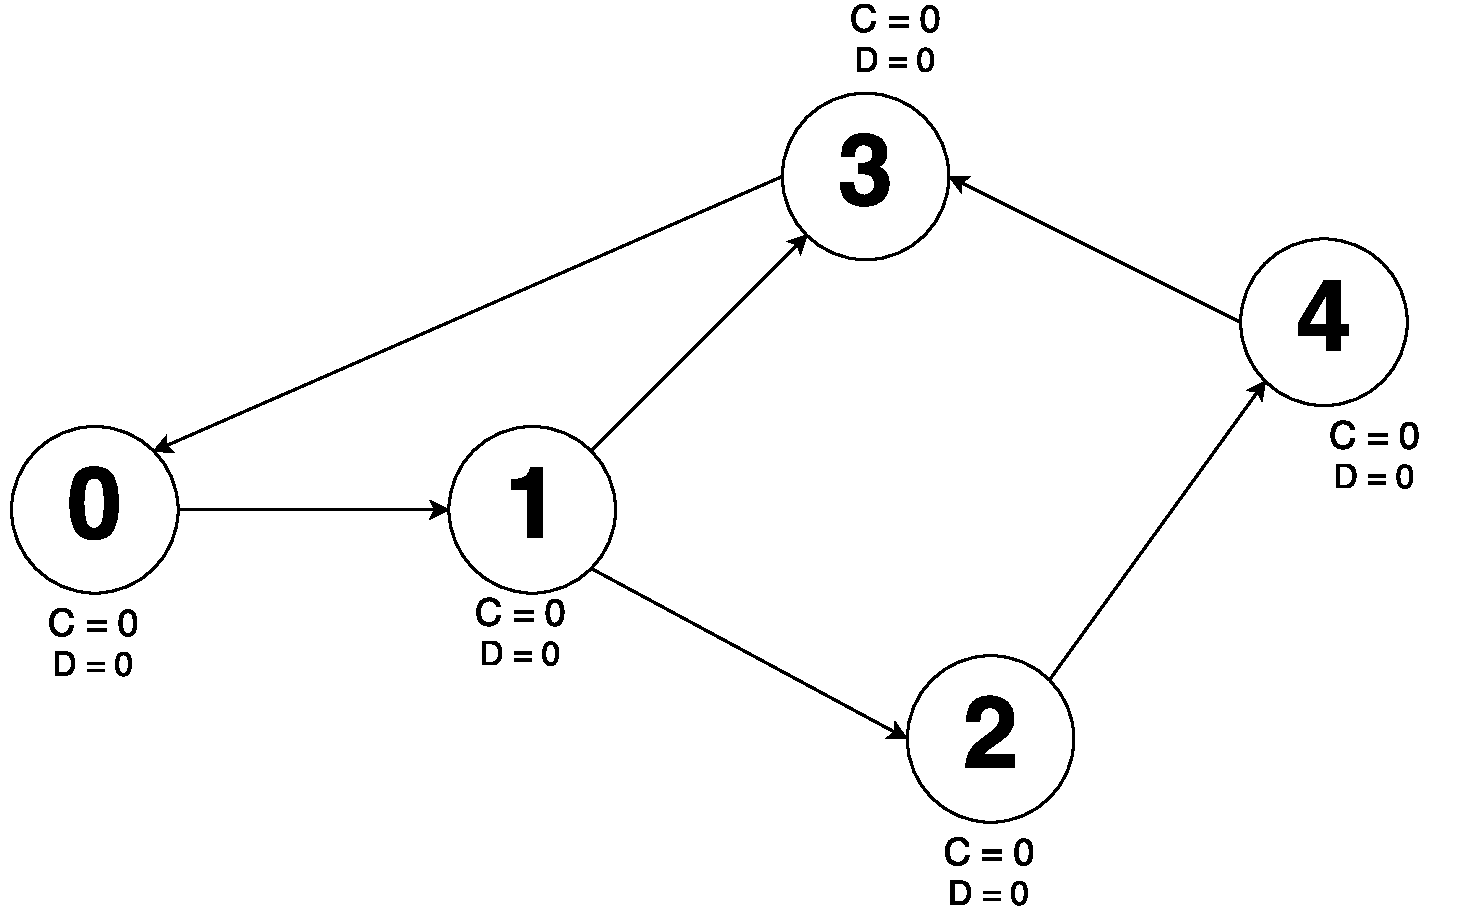
\includegraphics[width=\linewidth]{q2/10.pdf}
		\end{figure}
	
	
	

	
	
		
\end{document}